\section{积分的定义}
\label{sec:integ-definition}

黎曼积分把定义域切成小段，在每段上用一个高度近似函数。对有理点的指示函数$\mathbf 1_{\mathbb Q}$，任何小段上都同时有取$0$和取$1$的点，一个高度代表不了这一段。测度提供了另一种切法：按函数值把定义域分层，每一层是一个可测集合，层的高度乘以它的测度，再把各层相加。

图~\ref{fig:integ-slicing-comparison}把两种切法放在同一个函数上对比。左图的小矩形沿横轴并排，每个矩形对应定义域的一小段。右图取定一个值域区间$[t_k,t_{k+1})$，看哪些点的函数值落在其中：这些点在横轴上分成三段，彼此不相邻，却属于同一层。层的贡献只由高度和这三段的总长决定，三段分别在哪里无关紧要。

\begin{BookInlineFigure}
  \centering
  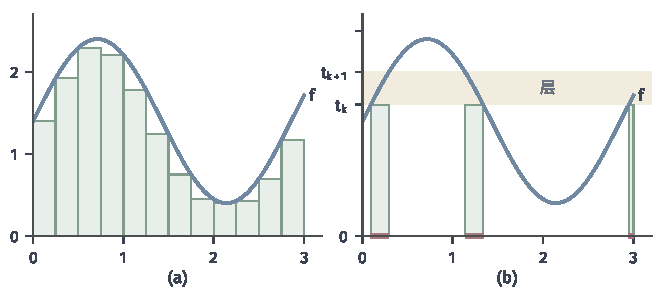
\includegraphics[width=112mm]{figures/04-spaces-measures-and-geometry/02-measure/matplotlib/integ-slicing-comparison/figure.pdf}
  \caption{同一函数$f(x)=1.4+\sin(2.2x)$的两种切法。(a)切定义域：把$[0,3]$等分成$12$段，绿色矩形以各段上$f$的下确界为高。(b)切值域：黄色带是值域区间$[1.6,2.0)$，红色线段是横轴上满足$1.6\leq f<2.0$的点，共三段，绿色矩形以$t_k=1.6$为高画在这些点上。}
  \label{fig:integ-slicing-comparison}
\end{BookInlineFigure}

下面先对只取有限个值的简单函数这样计算，再用简单函数从下方逼近一般的非负可测函数；随后用正负部分处理实值函数，用实部与虚部处理复值函数。

\subsection{非负积分}
\label{sec:integ-nonnegative}

\paragraph{简单函数的积分}
设$(X,\mathcal A,\mu)$是测度空间。非负简单函数在有限个不交可测集合上各取一个常值，分层已经现成，累计的方式就是“高度乘以测度”再求和。

由于测度可以为$+\infty$，先约定$0\cdot(+\infty)=0$：高度为零的层，无论占据多大的集合，贡献都是零。没有这条约定，$\mathbb R$上的零函数就没有积分。

\begin{definition}[非负简单函数的积分]
\label{def:integ-simple}
设$\varphi=\sum_{i=1}^mc_i\mathbf 1_{A_i}$是非负简单函数的标准表示，即$c_1,\dots,c_m\geq0$互不相同，$A_i=\{\varphi=c_i\}$。定义
\begin{equation}
 \int_X\varphi\,\mathrm d\mu=\sum_{i=1}^mc_i\,\mu(A_i)\in[0,+\infty].
 \label{eq:integ-simple}
\end{equation}
\end{definition}

图~\ref{fig:integ-simple-height}中$[0,3]$上的简单函数在$A_1=[0,1)\cup[2,2.5)$上取$2$，在$A_2=[1,2)\cup[2.5,3]$上取$0.5$。两层各占长度$1.5$，所以对Lebesgue测度的积分为
\[
 \int_{[0,3]}\varphi\,\mathrm d\lambda=2\times1.5+0.5\times1.5=3.75 .
\]
图下方的两行线段把两层在横轴上的位置单独画出。每一层都由不相邻的两段组成，而式~\eqref{eq:integ-simple}只用到它们的总长。

\begin{BookInlineFigure}
  \centering
  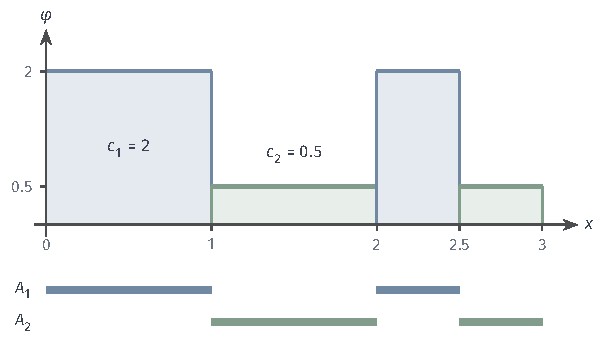
\includegraphics[width=102.401mm]{figures/04-spaces-measures-and-geometry/02-measure/tikz/integ-simple-height/figure.pdf}
  \caption{简单函数积分的“高度乘以测度”。$[0,3]$上的$\varphi$在$A_1=[0,1)\cup[2,2.5)$（蓝）上取$2$，在$A_2=[1,2)\cup[2.5,3]$（绿）上取$0.5$；下方两行线段标出两层占据的集合，各自总长为$1.5$。}
  \label{fig:integ-simple-height}
\end{BookInlineFigure}

同一个简单函数常常以别的方式写出，例如$[0,2]$的指示函数可以拆成$[0,1]$与$(1,2]$两段的指示函数之和。计算时我们希望随手把定义域切成方便的块，不必先合并成标准表示。下面的引理说明这样做得到同一个数，也给出简单函数积分的基本运算。

\begin{lemma}[简单函数积分的运算]
\label{lem:integ-simple-properties}
设$\varphi,\psi$是非负简单函数。
\begin{enumerate}
 \item 若$X$被分成两两不交的可测集$B_1,\dots,B_r$，$\varphi$在$B_j$上取常值$b_j$，则$\int\varphi\,\mathrm d\mu=\sum_jb_j\mu(B_j)$。
 \item 对$a,b\in[0,+\infty)$，有
 \begin{equation}
  \int(a\varphi+b\psi)\,\mathrm d\mu=a\int\varphi\,\mathrm d\mu+b\int\psi\,\mathrm d\mu .
  \label{eq:integ-simple-linear}
 \end{equation}
 \item 若$\varphi\leq\psi$，则$\varphi$的积分不超过$\psi$的积分。
 \item $E\mapsto\int\varphi\mathbf 1_E\,\mathrm d\mu$是$(X,\mathcal A)$上的测度。
\end{enumerate}
\end{lemma}

\begin{proof}
第1条。空的块对右端贡献为零，可以先去掉。设$\varphi$的标准表示为$\sum_ic_i\mathbf 1_{A_i}$，把取同一个值$c_i$的块合并，有
\[
 A_i=\bigcup_{j:\,b_j=c_i}B_j .
\]
由$\mu$的有限可加性，
\[
 \sum_jb_j\mu(B_j)=\sum_ic_i\sum_{j:\,b_j=c_i}\mu(B_j)=\sum_ic_i\mu(A_i).
\]

第2条。设$\varphi$的标准表示以$A_i$为块、取值$\alpha_i$，$\psi$的标准表示以$C_j$为块、取值$\beta_j$。集合$A_i\cap C_j$两两不交、并为$X$，$a\varphi+b\psi$在其上取常值$a\alpha_i+b\beta_j$。由第1条，
\[
 \int(a\varphi+b\psi)\,\mathrm d\mu=\sum_{i,j}(a\alpha_i+b\beta_j)\,\mu(A_i\cap C_j).
\]
把求和拆开，并对固定的$i$用有限可加性$\sum_j\mu(A_i\cap C_j)=\mu(A_i)$，对固定的$j$同样处理，得到
\[
 \int(a\varphi+b\psi)\,\mathrm d\mu=a\sum_i\alpha_i\mu(A_i)+b\sum_j\beta_j\mu(C_j).
\]

第3条。若$\varphi\leq\psi$，则在每个非空的$A_i\cap C_j$上$\alpha_i\leq\beta_j$。按这些块计算两个积分，再逐项比较即得。

第4条。函数$\varphi\mathbf 1_E$在$A_i\cap E$上取$c_i$，在$X\setminus E$上取$0$，由第1条，
\[
 \int\varphi\mathbf 1_E\,\mathrm d\mu=\sum_ic_i\,\mu(A_i\cap E).
\]
右端是有限个测度$E\mapsto\mu(A_i\cap E)$的非负加权和，由上一章的加权和规则，它是测度。
\end{proof}

\paragraph{一般非负函数的积分}
一般的非负可测函数可能取无穷多个值，没有有限分层可以直接计算。可行的办法是从下方逼近：若简单函数$\varphi$满足$0\leq\varphi\leq f$，它的积分就是$f$的累计的一个下界。上一章还证明了存在递增的简单函数列逐点趋于$f$，所以这些下界可以任意接近真正的累计。于是把全部下界的上确界定义为积分。

\begin{definition}[非负可测函数的积分]
\label{def:integ-nonnegative}
设$f:X\to[0,+\infty]$可测。定义
\begin{equation}
 \int_Xf\,\mathrm d\mu=\sup\Bigl\{\int_X\varphi\,\mathrm d\mu:\ \varphi\text{简单},\ 0\leq\varphi\leq f\Bigr\}.
 \label{eq:integ-nonnegative}
\end{equation}
值在$[0,+\infty]$中。常写作$\int f\,\mathrm d\mu$，或在不致混淆时写作$\int f$；对Lebesgue测度也写作$\int f(x)\,\mathrm dx$。
\end{definition}

这个定义与简单函数的积分不冲突。若$f$本身是简单函数，由引理~\ref{lem:integ-simple-properties}第3条，每个下方简单函数的积分都不超过$f$自己的积分，而$f$本身也是候选之一，所以上确界就是$f$自己的积分。

单调性可以直接从定义读出。若$0\leq f\leq g$，每个低于$f$的简单函数也低于$g$，上确界取在更大的范围上，于是$\int f\leq\int g$。

积分允许取$+\infty$。$\mathbb R$上$f\equiv1$的积分对Lebesgue测度为$\lambda(\mathbb R)=+\infty$。$(0,1]$上$f(x)=1/x$的积分也是$+\infty$：简单函数$\sum_{k=1}^nk\mathbf 1_{(1/(k+1),1/k]}$位于$f$下方，因为$(1/(k+1),1/k]$上$1/x\geq k$，而它的积分为
\[
 \sum_{k=1}^nk\Bigl(\frac1k-\frac1{k+1}\Bigr)=\sum_{k=1}^n\frac1{k+1},
\]
随$n$增大而无界。所以“积分有定义”与“积分有限”是两回事：非负函数的积分总有定义，但可能是$+\infty$。

\paragraph{递增逼近的积分}
定义用的是全部下方简单函数的上确界，这是一个庞大的集合。计算时我们只想用一列具体的逼近，例如上一章的二进分层逼近。下面的引理保证这样做不会漏掉任何下界。

\begin{lemma}[递增简单函数列的积分]
\label{lem:integ-increasing-simple}
设$f:X\to[0,+\infty]$可测，$\varphi_1\leq\varphi_2\leq\cdots$是非负简单函数，且对每个$x$有$\lim_n\varphi_n(x)=f(x)$。则
\begin{equation}
 \int_Xf\,\mathrm d\mu=\lim_{n\to\infty}\int_X\varphi_n\,\mathrm d\mu .
 \label{eq:integ-increasing-simple}
\end{equation}
\end{lemma}

\begin{proof}
积分$\int\varphi_n$关于$n$递增，并且都不超过$\int f$，所以极限存在且$\lim_n\int\varphi_n\leq\int f$。反方向要证明：对任意简单函数$0\leq s\leq f$，都有$\lim_n\int\varphi_n\geq\int s$。

固定$c\in(0,1)$，令$E_n=\{\varphi_n\geq cs\}$，它可测且关于$n$递增。下面说明$\bigcup_nE_n=X$。若$s(x)=0$，则$x\in E_1$。若$s(x)>0$，则$f(x)\geq s(x)>cs(x)$，而$\varphi_n(x)\to f(x)$，所以从某项起$\varphi_n(x)\geq cs(x)$。

由于$\varphi_n\geq cs\mathbf 1_{E_n}$，用单调性与线性性得到
\[
 \int\varphi_n\,\mathrm d\mu\geq c\int s\mathbf 1_{E_n}\,\mathrm d\mu .
\]
由引理~\ref{lem:integ-simple-properties}第4条，$E\mapsto\int s\mathbf 1_E\,\mathrm d\mu$是测度，集合$E_n$递增到$X$，所以由测度的从下连续性，右端趋于$c\int s\,\mathrm d\mu$。于是
\[
 \lim_n\int\varphi_n\,\mathrm d\mu\geq c\int s\,\mathrm d\mu .
\]
令$c\uparrow1$，得到所要的不等式。对$s$取上确界，即得$\lim_n\int\varphi_n\geq\int f$。
\end{proof}

引入因子$c<1$是为了处理$f(x)=s(x)$的点：在这些点上$\varphi_n(x)$可能永远略小于$s(x)$，却终究超过$cs(x)$。第~\ref{sec:integ-monotone-convergence}小节用一幅图看这件事，并把同一论证推广到一般的递增可测函数列。

\begin{example}[由定义计算$\int_{[0,1]}x\,\mathrm dx$]
\label{ex:integ-x-dyadic}
取$f(x)=x$，$x\in[0,1]$，测度为Lebesgue测度。二进分层逼近$\varphi_n$在$[k2^{-n},(k+1)2^{-n})$上取$k2^{-n}$，其中$0\leq k<2^n$；点$1$是零测集，在那里的取值不影响积分。每一层的宽度是$2^{-n}$，所以
\[
 \int\varphi_n\,\mathrm d\lambda=\sum_{k=0}^{2^n-1}\frac k{2^n}\cdot\frac1{2^n}=\frac1{4^n}\sum_{k=0}^{2^n-1}k .
\]
用等差数列求和$\sum_{k=0}^{2^n-1}k=\tfrac12(2^n-1)2^n$，得到
\[
 \int\varphi_n\,\mathrm d\lambda=\frac{(2^n-1)2^n}{2\cdot4^n}=\frac12\bigl(1-2^{-n}\bigr).
\]
前三项依次是
\[
 \frac14,\qquad\frac38,\qquad\frac7{16}.
\]
令$n\to\infty$，由引理~\ref{lem:integ-increasing-simple}得$\int_{[0,1]}x\,\mathrm dx=\frac12$，与黎曼积分的值相同。
\end{example}

图~\ref{fig:integ-dyadic-approx}画出了例子中的前三个逼近。绿色面积逐步填满直线下方的三角形。把第$n$步加细到第$n+1$步时，每个台阶右半边抬高$2^{-n-1}$，这些抬高部分的总面积是$2^{-n-2}$，正好是公式$\frac12(1-2^{-n})$的增量。

\begin{BookInlineFigure}
  \centering
  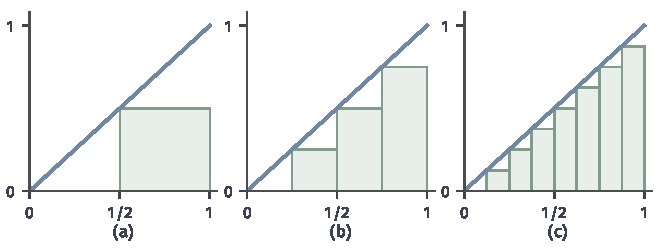
\includegraphics[width=112mm]{figures/04-spaces-measures-and-geometry/02-measure/matplotlib/integ-dyadic-approx/figure.pdf}
  \caption{$f(x)=x$（蓝）的二进分层逼近$\varphi_n$（绿色台阶）。(a)、(b)、(c)依次为$n=1,2,3$，绿色面积分别为$\frac14$、$\frac38$、$\frac7{16}$，递增趋于三角形面积$\frac12$。}
  \label{fig:integ-dyadic-approx}
\end{BookInlineFigure}

\paragraph{非负积分的可加性}
有了递增逼近，加法可以落到简单函数上完成。设$f,g$非负可测，取简单函数列$\varphi_n\uparrow f$与$\psi_n\uparrow g$，例如二进分层逼近。则$\varphi_n+\psi_n$是递增的非负简单函数，逐点收敛到$f+g$。由引理~\ref{lem:integ-increasing-simple}与引理~\ref{lem:integ-simple-properties}第2条，
\begin{equation}
\begin{aligned}
 \int(f+g)\,\mathrm d\mu&=\lim_n\int(\varphi_n+\psi_n)\,\mathrm d\mu\\
 &=\lim_n\int\varphi_n\,\mathrm d\mu+\lim_n\int\psi_n\,\mathrm d\mu\\
 &=\int f\,\mathrm d\mu+\int g\,\mathrm d\mu .
\end{aligned}
 \label{eq:integ-nonnegative-additive}
\end{equation}
用$c\varphi_n\uparrow cf$同样得到$\int cf=c\int f$，其中$c\in[0,+\infty)$。这些等式在$[0,+\infty]$中成立，允许两边为$+\infty$；系数取$+\infty$的情形放在第~\ref{sec:integ-linearity}小节核对。

\subsection{有符号积分}
\label{sec:integ-signed}

\paragraph{正部与负部}
取正负值的函数，正的贡献与负的贡献会相互抵消。若把两者混在一起累计，结果可能取决于累计的先后。最稳妥的做法是把两种贡献分开累计，最后再相减。对可测函数$f:X\to[-\infty,+\infty]$，令
\begin{equation}
 f^+=\max\{f,0\},\qquad f^-=\max\{-f,0\}.
 \label{eq:integ-parts}
\end{equation}
它们是非负可测函数，每一点至少一个为零，并且满足
\[
 f=f^+-f^-,\qquad \lvert f\rvert=f^++f^- .
\]
图~\ref{fig:integ-positive-negative-parts}以$\sin x$为例：$f^+$保留上半部分，$f^-$把下半部分翻到横轴上方。

\begin{BookInlineFigure}
  \centering
  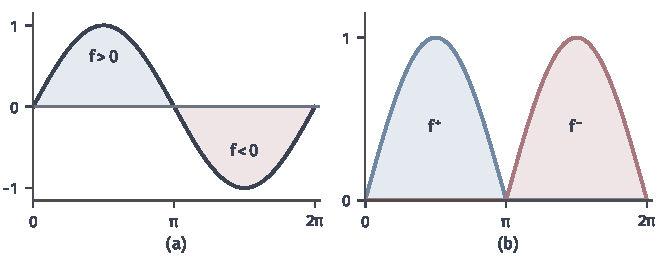
\includegraphics[width=112mm]{figures/04-spaces-measures-and-geometry/02-measure/matplotlib/integ-positive-negative-parts/figure.pdf}
  \caption{正负部分解，$f(x)=\sin x$，$x\in[0,2\pi]$。(a)$f$在$[0,\pi]$上为正（蓝底），在$[\pi,2\pi]$上为负（红底）。(b)正部$f^+$（蓝）与负部$f^-$（红）都是非负函数，每一点至少一个为零。}
  \label{fig:integ-positive-negative-parts}
\end{BookInlineFigure}

分开累计之后，两部分的积分都有意义，唯一的障碍是相减时可能出现$+\infty-(+\infty)$。下面的定义把这种情形排除在外。

\begin{definition}[积分存在与可积]
\label{def:integ-signed}
设$f:X\to[-\infty,+\infty]$可测。若$\int f^+\,\mathrm d\mu$与$\int f^-\,\mathrm d\mu$中至少一个有限，称$f$的积分存在，定义
\begin{equation}
 \int_Xf\,\mathrm d\mu=\int_Xf^+\,\mathrm d\mu-\int_Xf^-\,\mathrm d\mu\in[-\infty,+\infty].
 \label{eq:integ-signed}
\end{equation}
若$\int\lvert f\rvert\,\mathrm d\mu<+\infty$，称$f$关于$\mu$\term{可积}（integrable），也称\term{Lebesgue可积}（Lebesgue integrable），此时积分称为$f$的\term{Lebesgue积分}（Lebesgue integral）。
\end{definition}

三种情形可以这样区分。在$\mathbb R$上取$f=\mathbf 1_{[0,+\infty)}-\mathbf 1_{(-\infty,0)}$，正部与负部的积分都是$+\infty$，$f$的积分不存在；不能因为图像左右对称就说积分为零，那需要额外指定一种抵消的次序。取$f=\mathbf 1_{[0,+\infty)}$，积分存在且等于$+\infty$，但$f$不可积。取$f=\mathbf 1_{[0,1]}-\mathbf 1_{[-2,-1]}$，两部分的积分都是$1$，$f$可积且积分为$0$。

可积性用$\lvert f\rvert$规定，由$\lvert f\rvert=f^++f^-$与式~\eqref{eq:integ-nonnegative-additive}得
\[
 \int\lvert f\rvert\,\mathrm d\mu=\int f^+\,\mathrm d\mu+\int f^-\,\mathrm d\mu .
\]
所以$\int\lvert f\rvert<+\infty$当且仅当两部分的积分都有限。此时$\int f$是有限实数，并且
\[
 \Bigl\lvert\int f\,\mathrm d\mu\Bigr\rvert\leq\int f^+\,\mathrm d\mu+\int f^-\,\mathrm d\mu=\int\lvert f\rvert\,\mathrm d\mu .
\]

\paragraph{零测集与几乎处处等价类}
非负积分对零测集“视而不见”，这是用测度累计的直接后果：零测集这一层，高度再大，贡献也是零。下面的引理把这一点说清楚，并说明积分只依赖函数的几乎处处等价类。

\begin{lemma}[非负积分与零测集]
\label{lem:integ-null-sets}
设$f,g:X\to[0,+\infty]$可测。
\begin{enumerate}
 \item 对$t>0$，$\mu(\{f\geq t\})\leq\frac1t\int f\,\mathrm d\mu$。
 \item 若$\int f\,\mathrm d\mu<+\infty$，则$f<+\infty$几乎处处成立。
 \item $\int f\,\mathrm d\mu=0$当且仅当$f=0$几乎处处成立。
 \item 若$f=g$几乎处处成立，则$\int f\,\mathrm d\mu=\int g\,\mathrm d\mu$。
\end{enumerate}
\end{lemma}

\begin{proof}
第1条。$t\mathbf 1_{\{f\geq t\}}$是低于$f$的简单函数，它的积分是$t\mu(\{f\geq t\})$，所以$t\mu(\{f\geq t\})\leq\int f$。

第2条。对一切$t>0$有$\{f=+\infty\}\subseteq\{f\geq t\}$，由第1条，
\[
 \mu(\{f=+\infty\})\leq\frac1t\int f\,\mathrm d\mu .
\]
令$t\to+\infty$，右端趋于$0$。

第3条。若$\int f=0$，由第1条，对每个正整数$k$有$\mu(\{f\geq1/k\})=0$。又$\{f>0\}=\bigcup_k\{f\geq1/k\}$，所以$\mu(\{f>0\})=0$。反过来，设$N=\{f>0\}$零测。任一低于$f$的简单函数在$N$外为零，它的非零各层都含于$N$，测度为零，所以积分为$0$，上确界也是$0$。

第4条。设$N$是零测集，$f,g$在$N$外相等。对低于$f$的简单函数$\varphi$，函数$\varphi\mathbf 1_{X\setminus N}$低于$g$。由引理~\ref{lem:integ-simple-properties}第4条，
\[
 \int\varphi\,\mathrm d\mu=\int\varphi\mathbf 1_{X\setminus N}\,\mathrm d\mu+\int\varphi\mathbf 1_N\,\mathrm d\mu .
\]
最后一项按层计算为零，所以$\int\varphi\leq\int g$。对$\varphi$取上确界得$\int f\leq\int g$，对称地得到反向不等式。
\end{proof}

第1条称为\term{Markov不等式}（Markov inequality），它用积分控制函数取大值的集合有多大。在$[0,1]$上取$f(x)=x$、$t=\frac12$，左边是$\lambda(\{x\geq\frac12\})=\frac12$，右边是$2\cdot\frac12=1$，不等式成立。

对实值函数，若$f=g$几乎处处成立，则$f^\pm=g^\pm$几乎处处成立，由第4条，两者的积分存在性、可积性和积分值都相同。所以积分是定义在几乎处处等价类上的：在零测集上改动函数，或者在零测集上根本不给函数赋值，都不影响积分。

可积函数的取值可以是$\pm\infty$，但由第2条只能发生在零测集上，因此总可以改成处处取实数值的可积函数而积分不变。把可积函数按几乎处处相等分类，得到的空间及其范数结构在第~\ref{chap:function-normed-spaces}章研究。

\subsection{复值积分}
\label{sec:integ-complex}

\paragraph{复值可测函数的可积性}
Fourier分析中的$e^{\mathrm ikx}$、内积$\int\bar fg$都是复值的，所以积分要推广到复值函数。设$f=u+\mathrm iv:X\to\mathbb C$，其中$u,v$为实值可测函数，上一章已说明$\lvert f\rvert=\sqrt{u^2+v^2}$可测。复数没有正负之分，不能再用正部负部拆开；可以把它看成平面上的向量，分别累计两个坐标，而可积性仍用非负函数$\lvert f\rvert$规定。

\begin{definition}[复值函数的积分]
\label{def:integ-complex}
设$f=u+\mathrm iv$是复值可测函数。若$\int\lvert f\rvert\,\mathrm d\mu<+\infty$，称$f$可积，并定义
\begin{equation}
 \int_Xf\,\mathrm d\mu=\int_Xu\,\mathrm d\mu+\mathrm i\int_Xv\,\mathrm d\mu .
 \label{eq:integ-complex}
\end{equation}
\end{definition}

定义右端要求$u,v$都可积，下面的引理说明这正好由$\lvert f\rvert$可积保证。

\begin{lemma}[复值可积性的等价刻画]
\label{lem:integ-complex-integrable}
复值可测函数$f=u+\mathrm iv$可积，当且仅当$u$与$v$都可积。
\end{lemma}

\begin{proof}
平面上一个向量的长度不小于每个坐标的绝对值，不大于两个坐标绝对值之和，所以逐点有
\[
 \lvert u\rvert\leq\lvert f\rvert,\qquad\lvert v\rvert\leq\lvert f\rvert,\qquad\lvert f\rvert\leq\lvert u\rvert+\lvert v\rvert .
\]
若$\int\lvert f\rvert<+\infty$，由非负积分的单调性，$\int\lvert u\rvert$与$\int\lvert v\rvert$都有限。反过来，由单调性与式~\eqref{eq:integ-nonnegative-additive}，
\[
 \int\lvert f\rvert\,\mathrm d\mu\leq\int\lvert u\rvert\,\mathrm d\mu+\int\lvert v\rvert\,\mathrm d\mu<+\infty.
\]
\end{proof}

\paragraph{共轭与几乎处处相等}
复共轭$\bar f=u-\mathrm iv$与$f$的模相同，所以$\bar f$可积当且仅当$f$可积。由定义~\ref{def:integ-complex}直接得到
\[
 \int\bar f\,\mathrm d\mu=\int u\,\mathrm d\mu-\mathrm i\int v\,\mathrm d\mu=\overline{\int f\,\mathrm d\mu}.
\]
若复值函数$f,g$几乎处处相等，则实部、虚部分别几乎处处相等，由第~\ref{sec:integ-signed}小节，两者的积分相同。所以复值积分同样只依赖几乎处处等价类。

\begin{example}[复值积分的抵消]
\label{ex:integ-complex-cancel}
取$X=\{1,2,3,4\}$，每点质量$1/4$，$f(k)=\mathrm i^k$。实部$u$依次为$0,-1,0,1$，虚部$v$依次为$1,0,-1,0$。分别累计两个坐标：
\[
 \int u\,\mathrm d\mu=\frac14(0-1+0+1)=0,\qquad\int v\,\mathrm d\mu=\frac14(1+0-1+0)=0 .
\]
于是$\int f\,\mathrm d\mu=0$。另一方面$\lvert f\rvert\equiv1$，$\int\lvert f\rvert\,\mathrm d\mu=1$。四个方向的单位复数相互抵消，积分的模远小于模的积分。
\end{example}

复值积分把实值情形的运算搬到两个坐标上，不再比较大小。第~\ref{chap:function-inner-product-spaces}章的$L^2$内积$\langle f,g\rangle=\int f\bar g\,\mathrm d\mu$、第~\ref{chap:fourier-transform}章的Fourier系数与Fourier变换，都以这里的复值积分及其共轭规则为共同运算。
